\begin{figure}[H]
	\centering
	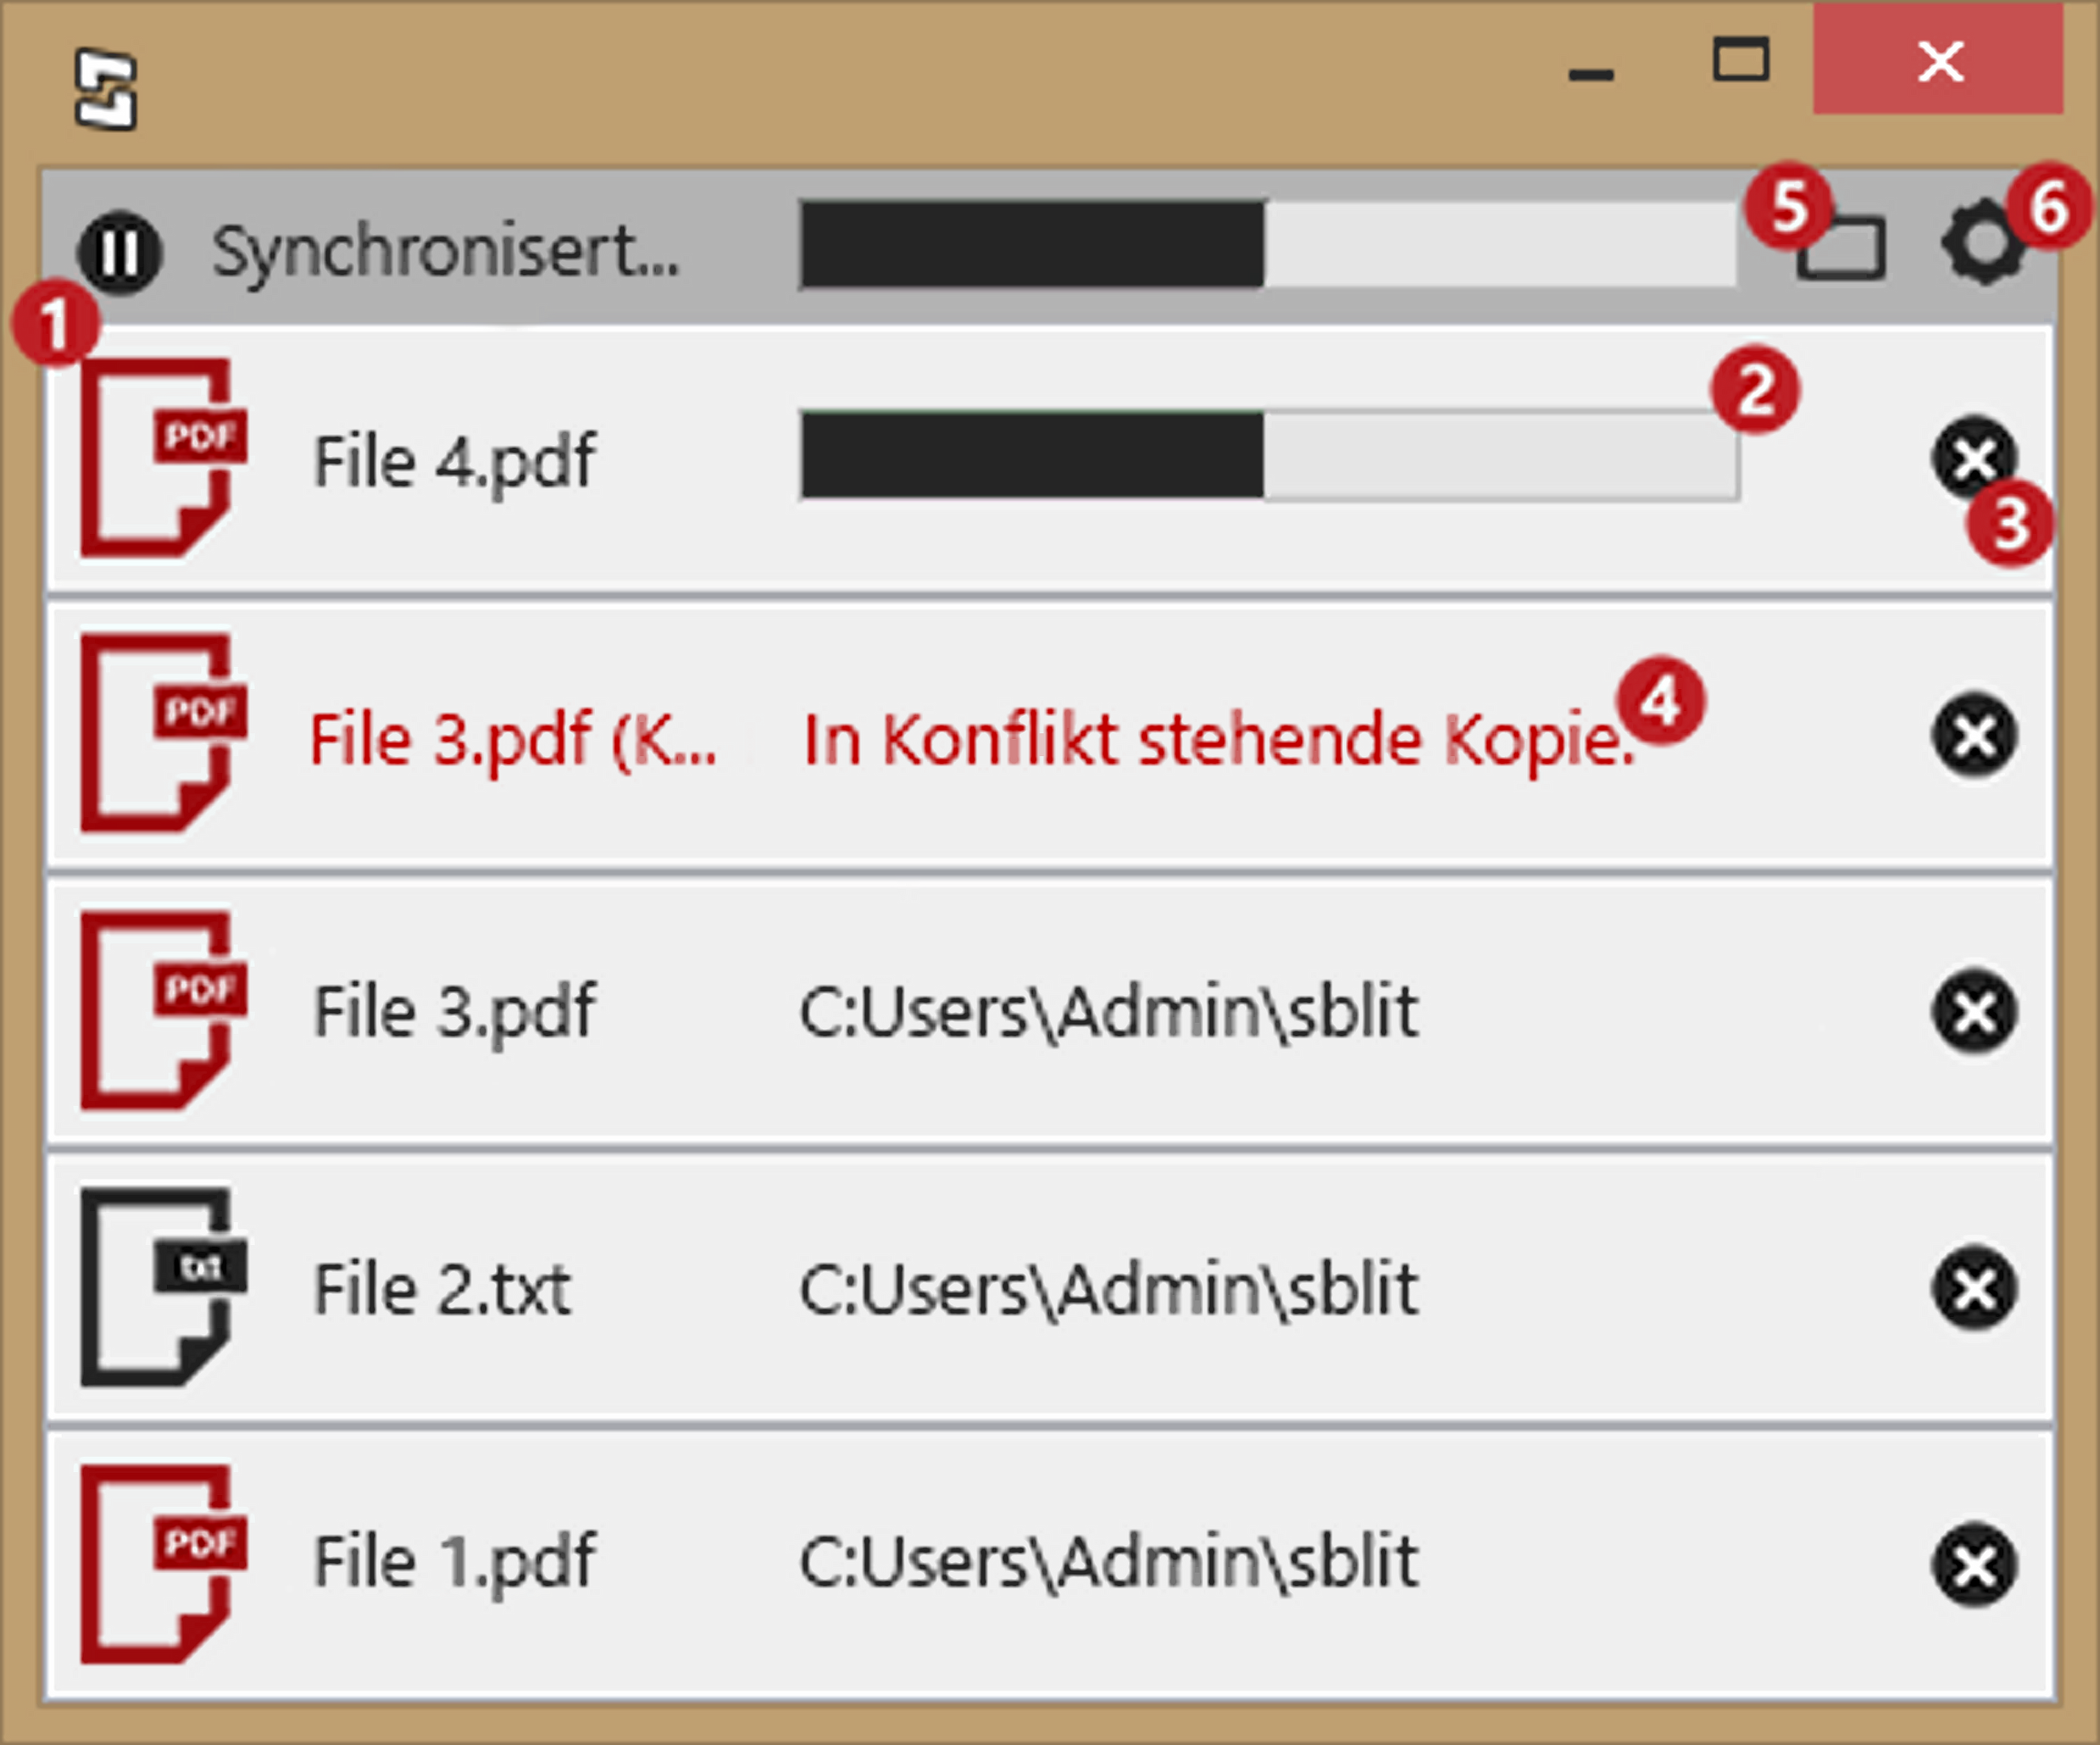
\includegraphics[scale=0.7]{images/ueberblicksfenster.png}
  \caption{Überblicksfenster}
	\label{ueberblicksfenster}
\end{figure}

Mit einem einfachen Klick auf das Icon im System-Tray öffnet sich das Überblicksfenster, in der der
Benutzer auf die folgenden Optionen Zugriff bekommt:

\begin{description}

	\descriptionitem{Letzte Änderungen innerhalb des sblit-Ordners}
		Dem Benutzer wird hier eine Auflistung der zuletzt hinzugefügten Dateien
		geboten. Neben dem an den Dateityp angepassten Bild wird auch der Dateiname
		und Ordnerpfad angegeben.

	\descriptionitem{Fortschrittsbalken laufender Synchronisationsvorgänge}
		Bei laufenden Synchronisationen hat der User die Möglichkeit, den
		Fortschritt zu verfolgen.

	\descriptionitem{Button für das Abbrechen der Synchronisation}
	  Beispielsweise nach irrtümlichem Hinzufügen von Dateien, hat der Benutzer die
		Möglichkeit, die laufende Synchronisation mithilfe des Abbrechen-Buttons
		abzubrechen.

	\descriptionitem{Anzeige von aufgetretenen Fehlern}
		Bei \glspl{syncconflict}n, die auftreten, wenn zwei \glspl{syncpartner} die
		selbe Datei gleichzeitig bearbeiten, sowie bei diversen anderen Fehlern,
		wird der User benachrichtigt.

	\descriptionitem{Link zum sblit-Ordner}
		Um dem Benutzer schnellen Zugriff auf seinen konfigurierten sblit-Ordner zu
		gestatten, gibt es den Ordner-Button, mit dem sich der sblit-Ordner im
		Datei-Browser öffnet.

	\descriptionitem{Öffnen des Konfigurationsmenüs}
		Mit einem Klick auf den Optionen-Button öffnet sich das Konfigurationsmenü,
		welches im folgenden Abschnitt gezeigt wird.
\end{description}
